
%%%%%%%%%%%%%%%%%%%%%%% paper_sem_web.tex %%%%%%%%%%%%%%%%%%%%%%%%%
%
% This is the LaTeX source for the instructions to authors using
% the LaTeX document class 'llncs.cls' for contributions to
% the Lecture Notes in Computer Sciences series.
% http://www.springer.com/lncs       Springer Heidelberg 2006/05/04
%
% It may be used as a template for your own input - copy it
% to a new file with a new name and use it as the basis
% for your article.
%
% NB: the document class 'llncs' has its own and detailed documentation, see
% ftp://ftp.springer.de/data/pubftp/pub/tex/latex/llncs/latex2e/llncsdoc.pdf
%
%%%%%%%%%%%%%%%%%%%%%%%%%%%%%%%%%%%%%%%%%%%%%%%%%%%%%%%%%%%%%%%%%%%


\documentclass[runningheads,a4paper]{llncs}
\usepackage[ngerman]{babel}
\usepackage[pdftex]{graphicx}
\usepackage[utf8x]{inputenc}
\usepackage[T1]{fontenc} 
\usepackage{mathtools}
\usepackage{amsfonts,amsmath,amssymb}
\usepackage{wasysym}
\usepackage{natbib}

\setcounter{tocdepth}{3}
\usepackage{url}

\usepackage{listings}
\usepackage{chngcntr}
\AtBeginDocument{\counterwithout{lstlisting}{section}}



\usepackage{xcolor}  
\definecolor{grey}{rgb}{0.5,0.5,0.5}
\lstdefinelanguage{ttl}{
sensitive=true,
morecomment=[l][\color{grey}]{@},
morecomment=[l][\color{black}]{\#},
morestring=[b][\color{black}]\",
numbers=left,
%frame=shadowbox,
basicstyle=\scriptsize\ttfamily,
tabsize=2,
}     

\definecolor{codegreen}{rgb}{0,0.6,0}
\definecolor{codegray}{rgb}{0.5,0.5,0.5}
\definecolor{codepurple}{rgb}{0.58,0,0.82}
\definecolor{backcolour}{rgb}{0.95,0.95,0.92}
 
\lstdefinestyle{mystyle}{
    backgroundcolor=\color{backcolour},   
    commentstyle=\color{codegreen},
    keywordstyle=\color{magenta},
    numberstyle=\tiny\color{codegray},
    stringstyle=\color{codepurple},
    basicstyle=\footnotesize,
    breakatwhitespace=false,         
    breaklines=true,                 
    captionpos=b,                    
    keepspaces=true,                 
    numbers=left,                    
    numbersep=5pt,                  
    showspaces=false,                
    showstringspaces=false,
    showtabs=false,                  
    tabsize=2
}
 
\lstset{style=mystyle}

\urldef{\mailsa}\path|manuel.b.dudda@student.hs-rm.de|    
\newcommand{\keywords}[1]{\par\addvspace\baselineskip
\noindent\keywordname\enspace\ignorespaces#1}

\begin{document}

\mainmatter  % start of an individual contribution

% first the title is needed
\title{Schließen auf Usability-Probleme mit OWL 2 RL}

% a short form should be given in case it is too long for the running head
% \titlerunning{Schließen auf Usability-Probleme mit OWL 2 RL}

% the name(s) of the author(s) follow(s) next
%
% NB: Chinese authors should write their first names(s) in front of
% their surnames. This ensures that the names appear correctly in
% the running heads and the author index.
%
\author{Manuel Dudda}
%
% \authorrunning{Schließen auf Usability-Probleme mit OWL 2 RL}
% (feature abused for this document to repeat the title also on left hand pages)

% the affiliations are given next; don't give your e-mail address
% unless you accept that it will be published
\institute{Hochschule RheinMain Informatik Master of Science \\
Fachbereich Design Informatik Medien \\
Campus Unter den Eichen 5
65195 Wiesbaden , Deutschland\\
\mailsa\\
\url{https://github.com/manuel84/abrupt}}

%
% NB: a more complex sample for affiliations and the mapping to the
% corresponding authors can be found in the file "llncs.dem"
% (search for the string "\mainmatter" where a contribution starts).
% "llncs.dem" accompanies the document class "llncs.cls".
%

\toctitle{Lecture Notes in Computer Science}
\tocauthor{Authors' Instructions}
\maketitle

\renewcommand{\abstractname}{Abstract}
\begin{abstract}
Die Usability von Internetauftritten wird größtenteils subjektiv wahrgenommen. 
Es existiert zwar eine Normierung durch die ISO für die Anforderungen an die Gebrauchstauglichkeit einer Software (EN ISO 9241-11), diese trifft jedoch nur sehr wage Aussagen und orientiert sich stark am respektiven Nutzungskontext. 
Trotzdem gibt es Merkmale einer Website, die allgemein als negativ für die Eigenschaften der Usability eingestuft werden können, so zum Beispiel schlechte Kontrastverhältnisse, ein hoher Lesbarkeitsindex und Diskrepanzen zwischen erwartetem und tatsächlichem Nutzerverhalten. 
Das "{}AbRUPt"{}-System der Hochschule RheinMain ist in der Lage viele dieser Merkmale einer Website automatisiert zu erfassen. 
Durch die Konvertierung, Modellierung und Entwicklung eines durchdachtes Regelsystem in der semantischen Ontologiesprache OWL 2 RL ensteht ein System, welches automatisiert Folgerungen auf Usability-Probleme ermöglicht.
\end{abstract}

\newpage

\section{Einleitung}
Die Gestaltungsvielfalt von Webseiten hat sich seit der Freigabe des Internets für die kommerzielle Nutzung (ca. 1990) rasant weiterentwickelt. 
Anfangs bot nur eine kleine Anzahl von Institutionen, Firmen, Regierungen spärliche Informationen meist im Form von einfachen Texten an. 
Mittlerweile gehört die Webseite zum Aushängeschild eines jeden Unternehmens. 
Das Aussehen muss dabei häufig zur Unternehmensphilosphie passen, das sogenannte Cooperate Design sorgt für eine visuelle Identität, um sich von anderen Unternehmen zu unterschieden. 
Dazu gehören Schriftbild, Farben, Logos, und vieles mehr.
Des Weiteren wurden jede Menge Web-Dienste entwickelt, die den Webseiten mehr Interaktivität einräumen. 
Webanwendungen ähneln komplexer Software, die eine grafische Benutzeroberfläche im Browser zur Verfügung stellen.
Für die Benutzerfreundlichkeit gibt es eine ISO-Norm, die folgende Anforderungen an die Software stellt:

\begin{quote}
Die Gebrauchstauglichkeit einer Software ist von ihrem Nutzungskontext (beinhalten den Benutzer, die Arbeitsaufgabe, die Arbeitsmittel wie z.B. Hardware oder Software sowie die physische und soziale Umgebung) abhängig, in dem sie eingesetzt wird. 
Im Teil 11 der ISO 9241 werden drei Leitkriterien für die Gebrauchstauglichkeit einer Software bestimmt:
\begin{itemize}
\item{Effektivität zur Lösung einer Aufgabe,}
\item{Effizienz der Handhabung des Systems,}
\item{Zufriedenheit der Nutzer einer Software.}
\end{itemize}


\end{quote}

Es wird deutlich, dass es keine objektive Bestimmung von Gebrauchstauglichkeit gibt, sondern diese stark vom Nutzungskontext abhängt. 
Insbesondere spielt die Zielgruppe dabei eine Rolle. 
Handelt es sich um ein jüngeres Publikum, die man mit einfacher Sprache zu erreichen versucht oder um Fachpublikum, für die komplexere Texte unabdingbar sind?
Welche kulturellen Gegebenheiten sind zu beachten? 
Das Farbverständnis der Chinesen beispielweise weicht der westlichen Welt stark ab, so ist weiß die Farbe der Trauer.
Ob eine Software dementsprechend gebrauchstauglich ist oder nicht, ist demnach nur subjektiv von Menschen bewertbar.
Dennoch gibt es auch Merkmale, die allgemeingültig als mögliche Probleme eingestuft werden können:

\begin{itemize}
\item{Schlechte Kontrastverhältnisse}
\item{Seiten ohne/mit zu vielen Links}
\item{Unausgeglichenes Bild/Text-Verhältnis}
\item{Diskrepanzen zwischen erwarteter und tatsächliher Formular-Eingabezeiten}
\item{Texte mit schlechtem Lesbarkeitsindex anhand \cite{lesbarkeit}}
\item{Inkonsistenzen in der HTML-Struktur}
\end{itemize}

Der Online-Service AbRUPt \cite{abrupt} von der Hochschule RheinMain bietet die Möglichkeit viele dieser Merkmale über eine Web-Schnittstelle zu erfassen. 
In \cite{Brieger} wurde gezeigt, wie man diese Schnittstelle anwendet und daraus ein Konstrukt für eine mögliche Datenauswertung entwickelt.
Diese Arbeit beschäftigt sich mit der Weiterentwicklung des darin beschrieben Converters und dessen Datenuswertung (Abb. \ref{fig:converter}).

\begin{figure}
\caption{Funktionsweise des Converters}
\centering
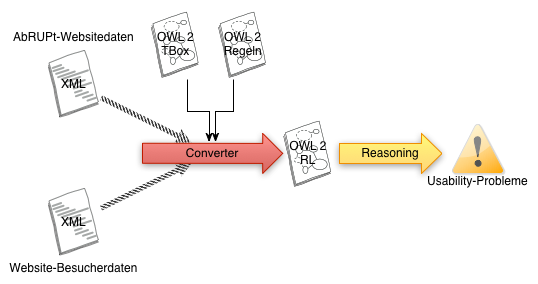
\includegraphics[width=0.7\textwidth]{figures/converter}
\label{fig:converter}
\end{figure}

Die Daten liegen zunächst im XML-Format vor und werden in OWL konvertiert.
Mittels OWL-basierter Regeln wird überprüft, ob eine aussagekräftige Datenauswertung möglich ist.
Es wird dabei besonderer Wert auf das OWL-Profil {}"RL{}" gelegt, um Performance-Schwachstellen zu vermeiden.
Das OWL 2-RL Profil basiert auf dem funiderten Grundlagen der Beschreibungslogiken (\ref{sec:desclogic}).

\section{Gliederung}
\label{sec:structure}

Im Abschnitt \ref{sec:logic} werden die theoretischen Grundlagen für das OWL 2 RL-Profil aufgearbeitet. 
Um zu verstehen, wie sich eine Beschreibungslogik (\ref{sec:desclogic}) von der Aussagenlogik (\ref{sec:aussagenlogik}) abhebt werden kurze Beispiele gezeigt, wie sie auch in der Anwendung existieren könnten.
Abschnitt \ref{sec:prediactelogic} zeigt, dass mächtigere Aussagen mit der Prädikatenlogik möglich sind und welche Einschränkungen in der Entscheidbarkeit daraus entstehen.
Insgesamt stellt die Implementierung (\ref{sec:implementation}) des Converters eine Erweiterung vorheriger Arbeiten dar.
Welche Anpassungen dabei vorgenommen wurden wird in Abschnitt \ref{sec:customization} beschrieben, welche Technologien in \ref{sec:technology}.
Der wesentliche Bestandteil der Erweiterung besteht aus der Regelerstellung für das Schließen auf Probleme (\ref{sec:reasoning}).
Die Regeln sind in Inkonsistenz- (\ref{sec:rule_inconsistency}), Produktions- (\ref{sec:rule_production}), Listen- \ref{sec:rule_list} und Datentyp-Regeln (\ref{sec:rule_datatype}) unterteilt.
Einige Herausforderungen können nur durch den Einsatz von Erweiterungen beschrieben in \ref{sec:rule_extensions} gelöst werden.
Verbundene Arbeiten werden in Abschnitt \ref{sec:related_work} erwähnt.
Abschließend wird das Projekt in \ref{sec:conclusion} zusammengefasst, ein Ausblick gewährt sowie ein persönliches Fazit gezogen.

\newpage
\section{Logik und Berechenbarkeit}
\label{sec:logic}

Es gibt verschiedene Arten von formalen Logiken, die sich in ihrer Struktur und Mächtigkeit unterscheiden.
Für triviale Anwendungsfälle reicht meistens die Verknüpfung von strukturlosen Elementaraussagen aus.
Komplexere Aussagen lassen sich nur mit mächtigeren Logiken ausdrücken, für dessen automatiserten Schlussfolgerungen allerdings auch größere Aufwände entstehen.

\subsection{Aussagenlogik}
\label{sec:aussagenlogik}

Mit der Aussagenlogik lassen sich in ihrer Mächtigkeit beschränkte Formeln aufstellen \cite[p. 6,373]{foundations}. Sie entsprechen in der Programmierung dem Datentyp \textit{Boolean}, also Elementarussagen, die verknüpft und negiert erscheinen und deren Wahrheitsgehalt \textit{Wahr} oder \textit{falsch} ist.

\begin{figure}
\begin{align}
\begin{split}
A &= \textnormal{Die Checkbox hat den Namen \textit{agb}.}\\
B &= \textnormal{Die Checkbox ist kein Pflichtfeld.}\\
A \to C &= \textnormal{Die Checkbox hat den Namen \textit{agb}, also ist sie ein Pflichtfeld.}\\
(A \to C) \land B &= \textnormal{\lightning\ (Es liegt ein Problem vor.)}
\label{eq:propositional_logic}
\end{split}
\end{align}
\caption{Aussagenlogische Formeln}
\end{figure}
 
Aus den oben genannten Aussagen \eqref{eq:propositional_logic}, folgt, dass die Checkbox mit dem Namen \textit{agb} ein Pflichtfeld ist (\(A \to C)\). 
Diese ist allerdings nicht als solches ausgezeichnet (\(B\)). 
Aus dieser Inkonsistenzeigenschaft ergibt sich ein Problem (\(A \to C) \land B\). 
Die Aussage \((A \to C)\) könnte genauso als die Negation von \(B\) definiert werden. 
Es ergäbe sich daraus eine Kontradiktion \((\neg B \land B)\), einer Formel die stets zu \textit{falsch} ausgewertet wird. 
Über Wahrheitstafeln können jegliche (zusammengesetzte) Aussagen auf deren Wahrheitsgehalt überprüft werden. 
Damit verdeutlicht sich einfach, dass das Schlussfolgern über die aussagenlogische Formeln ein entscheidbares Problem darstellt.
\\

\subsection{Prädikatenlogik}
\label{sec:prediactelogic}

Eine Erweiterung der Aussagenlogik stellt die Prädikatenlogik dar \cite[p. 6,367--373]{foundations}.
In der Prädikatenlogik werden Elementaraussagen hinsichtlich ihrer Struktur untersucht.
Mit Prädikaten können Eigenschaften über Individuen festgelegt werden. 
Die Anzahl der Stellen im Prädikat ist dabei nicht beschränkt, so können mit 1-stelligen Prädikaten Zugehörikeiten \eqref{eq:fol_predicate1}, mit 2-stelligen Rolleneigenschaften \eqref{eq:fol_predicate1} modelliert werden  
Quantoren geben an, von wie vielen Individuen eine Aussage erfüllt wird, so kann die Aussage über die Existenz eines Individuums getroffen werden \eqref{eq:fol_quantors}.
% \renewcommand{\figurename}{Fig.}
\begin{figure}
\begin{equation}
TextInput(x)
\label{eq:fol_predicate1}
\end{equation}
\caption{Prädikatenlogik erster Stufe: 1-stelliges Prädikat als Klasse}
\end{figure}

\begin{figure}
\begin{equation}
hasName(x, \textnormal{agb})
\label{eq:fol_predicate2}
\end{equation}
\caption{Prädikatenlogik erster Stufe: 2-stelliges Prädikat als Rolleneigenschaft}
\end{figure}

\begin{figure}
\begin{equation}
\forall x\exists y. TextInput(x) \to hasName(x, y)
\label{eq:fol_quantors}
\end{equation}
\caption{Prädikatenlogik erster Stufe: Quantoren als Existenz-Aussagen}
\end{figure}

Somit lassen sich wesentlich mächtigere Aussagen treffen, die mit der Aussagenlogik allein nicht möglich sind.
Das hat allerdings auch Asuwirkungen auf die Laufzeit des Schlussfolgerns.
Das Entscheidungsverfahren für die Prädikatenlogik ist unentscheidbar. 
\\

\subsection{Beschreibungslogiken}
\label{sec:desclogic}

Eine entscheidbare Untermenge der Prädikatenlogik erster Stufe bieten die Beschreibungslogiken \cite{foundations}.
Im Wesentlichen enthält eine Beschreibungslogik die Operatoren der Aussagenlogik (\(\land, \lor, \neg\)), ein- und zweistellige Prädikate sowie eine eingeschränkte Quantifizierung.
Sie umfassen Individuen (Objekte), Rollen (2-stellige Prädikate) und Klassen (1-stellige Prädikate), wobei keine Metamodellierung (Klassen von Klassen) möglich ist.
Normalerweise wird die Wissensbasis dabei in 2 Teile separiert, \textit{TBox} und \textit{ABox}. 
Das Terminoligische Wissen (\textit{TBox}) beschreibt die Struktur möglicher Welten. 
Es stellt Begriffe zur Beschreibung von Sachverhalten bereit. 
So definiert es das Vokabular in einem Anwendungsbereich. 
Das Grundvokabular besteht aus den Klassen (einstellige Prädikate) und Rollendefinitionen (zweistellige Prädikate). 
Das Assertionale Wissen beschreibt die Sachverhalte, die in einer bestimmten Welt gelten. 
Es existieren Annahmen (assertions) über einzelne Objekte ausgedrückt mit
Hilfe des Grundvokabulars.

Die Syntax ist stark an die Prädikatenlogik angelehnt. 
Es gibt jedoch wesentliche Unterschiede. 
Hervorzuheben ist der Wegfall der Implikation (\(\to\)). 
Während in der Prädikatenlogik auch Rollenaxiome rechterhand der Implikation stehen können (\eqref{eq:fol_predicate1}), sind bei Beschreibungslogiken nur Klassen in Subsumptionen möglich \(C_1 \sqsubseteq C_2\).
Nur ein Teil der Prädikatenlogik ist demnach adäquat in eine Beschreibungslogik zu übersetzen, man spricht in diesem Fall von DL-safe Regeln. 

Eine Auflistung der Syntax und der Entsprechung in Prädikatenlogik sowie OWL finden Sie in \ref{table:description_logic}.
\\
Mit dem RL-Profil aus OWL 2 \cite{owl2rl} gibt es eine Sprache, die die gleiche Mächtigkeit wie die Beschreibungslogik (\(\mathcal{SHOIN}(D))\) besitzt und demnach für das Reasoning in entscheidbarer Komplexität bestens geeignet ist.
Sie hat ein gute Balance zwischen Ausdrucksfähigkeit und Berechenbarkeits-/Verarbeitungseigenschaften.
OWL 2 ist zu dem Empfehlung des W3C und es existieren bereits einige Reasoner-Implementierungen. 
Die bekanntesten derzeit sind Fact++, Hermit, KAON2 und Pellet.


\section{Implementierung}
\label{sec:implementation}

\cite{Brieger} untersuchte inwieweit das Analyse-Tool \cite{abrupt} verwendet werden kann um eine objektive Beurteilung über die Benutzerfreundlichkeit einer Webseite geben zu können. 
Die Arbeit zeigt gute Ansätze und setzt auf die Konvertierung der erhobenen Daten in ein OWL-Dokument. 
Mit einem anschließenden Projekt können mit einem durchdachten Regelsystem Schlussfolgerungen gezogenwerden. 
Das Programm ist als Dienst mit HTML-Oberfläche gestaltet und kann lediglich die Webseiten-Daten aus \textit{AbRUPt} umwandeln, die Integration der Webseiten-Besucherdaten ist noch nicht berücksichtigt. 
Auch die Integration in nachfolgende Projekte erweist sich durch den wenig modularen Aufbau als eher schwierig. 
Mit Einbezug der Ergebnisse aus \cite{Martin} konnte ein Konzept für eine sinnvolle Aufbereitung der Daten gezeigt werden. 
Es ist OWL-Converter entstanden, der erhobene \textit{AbRUPt}-Daten von einem XML-Format in ein OWL-Dokument transformiert.

\subsection{Anpassungen und Erweiterung des OWL-Converters}
\label{sec:customization}

Einige wichtige Aspekte wurden gegenüber dieser Arbeit geändert. 
Die Ontologie für den \textit{AbRUPt-Service} wurde von Grund auf intuitiver gestaltet und um die Konzepte der Webseiten-Besucherdaten erweitert (\ref{fig:onto}). 
Dabei wurde ebenso auf sinnvolle Konsistenzeigenschaften sowie Inferenz-Regeln zurückgegriffen, die auf Usabilty-Probleme schlussfolgern. (\ref{sec:reasoning})
Ein Problem ergab sich für die Eindeutigkeit von Webseiten-Elementen, die nicht kontextbasiert benannt wurden. 
Mit dem an \textit{REST} \cite{rest} angelehnten URI-Aufbau ergeben sich global einheitlich URIs.
Dabei wird der Kontext in die URI-Struktur jeweils eingebettet (Listing \ref{listing:nested_uris}). 
Ein Formular-Element kann somit auf mehreren Webseiten mit gleicher Id, Name und sonstigen Attributen koexistieren und wird nicht zu dem selben OWL-Element konvertiert. 
Beispielsweise liegt dann das Input-Textelement des Namens für ein Kontaktformular innerhalb von Formular (Form = \textit{kontaktformular}), Seitenstatus (State = \textit{state5}), Seiten-URL (Page = \textit{http://www.rikscha−mainz.de/Kontakt}) und der zugehörigen Website (Website = \textit{http://www.rikscha−mainz.de}).
Das sieht zunächst nicht sehr lesbar aus, ist aber unvermeidbar aufgrund möglicher großer Datenbestände. 

\lstinputlisting[breaklines=true,language=ttl, caption=Nested URIs, label=listing:nested_uris]{listings/unique_nested_uris.ttl}
 
Für die Einstufung von Problemen gibt es die Klasse \textit{Problem}. 
Durch geeignete Abfragen, bspw. mit SPARQL \ref{sparql}, kann nach dem Reasoning die Liste aller möglichen Probleme abgerufen werden. 
Wie bereits angesprochen können dabei Elemente dazugehören, die aus einem subjektiven Erscheinungsbild annehmbar als Problem ignoriert werden können.

\subsection{Eingesetzte Technologien}
\label{sec:technology}

Für die Neugestaltung des Konvertierung-Tools fiel die Wahl der Technolgie auf \textit{RubyGems}, dem offiziellen Paketsystem von Ruby . 
Zum einen ist die Unterstützung durch ruby-rdf \cite{ruby-rdf} für RDF/OWL ausgezeichnet und zum Anderen erweisen sich noch weitere wesentliche Vorteile:
\begin{itemize}
    \item{Benutzung durch Kommandozeilentool}
    \item{Modularer Aufbau}
    \item{Ausgezeichnete Komponententest-Unterstützung}
    \item{Wiederverwendbarkeit durch Einbindung als RubyGem Bibliothek oder des Kommandozeilentools}
    \item{Flexibilität der Eingabe und Ausgabe (bestimmte Services, nur Abrupt/ohne Benutzerdaten, tutrle, rdfxml, n3}
\end{itemize}

Das terminologische Wissen (TBox) ist in einem OWL-Dokument gesichert, sodass es separat mit Protege entwickelt und in die Software einfach eingebunden wird. 
Da es sich ausschließlich um statische Inhalte handelt, erweist sich dies als sinnvoll. 
Zur Hervorhebung und Veranschaulichung von nicht-trivialen Regeln existieren weitere OWL-Dokumente, die als Ordnerinhalte der Software hinzugefügt werden. 
Mit dem Befehl in Listing \ref{listing:cli} lässt sich Konvertierung starten. 
Zunächst werden die statischen Inhalten in ein RDF-Repsoitory geladen. 
Das Assertionale Wissen (ABox) entsteht aus der Transformation der Eingabedaten. 
Die Eingabedaten liegen in der Regel in 2 XML-Dokumenten vor - den Website- und den Besucher-Daten.
Für jeden Kontentyp existiert eine Schema-Datei, die für die nötige Datentypkonvertierung sorgt. 
Dadurch werden aus den XML-Rohdaten die nötigen Werte umgewandelt, bspw. Integer, Date, Decimal, ...
Anschließend erstellt eine zugewiesene Transformater-Klasse aus den XML-Daten die RDF-Statements zu dem RDF-Repository hinzu. 
Der Aufbau der Software ist somit sehr modular, individuell anpassbar, durch Oberklassen generisch und übersichtlich.

\newpage

\section{Schließen auf Probleme mit Inferenz-Regeln}
\label{sec:reasoning}

Die formale Beschreibungssprache OWL 2 ist eine Empfehlung des W3C \cite{owl2} vom 11. Dezember 2012 für die Beschreibung von Ontologien. 
Primär geht es darum Modellierungen einer Weltanschauung (Domäne) vorzunehmen, sodass Mensch und Maschine die Bedeutung verarbeiten können. 
OWL 2 basiert technisch auf RDF und RDFS und geht dabei über die Ausdrucksmächtigkeit weit hinaus. 
Es ist dokumentenbasiert, was die Erstellung und Verteilung gegenüber einem Binärformat enorm vereinfacht. 
Um die richtige Balance zwischen Ausdrucksstärke und Entscheidbarkeit bzw. Performance zu gewährleisten gibt es 3 verschiedene Sprachebenen - Lite, DL und Full. 
In dieser Arbeit wird der Fokus auf die 2. Sprachebene OWL 2 DL gelegt, für welche es 3 Profile existiert. 
Das OWL 2 RL Profil ist auf Anwendungen, die ein skalierbares Reasoning verlangen, ohne dabei zu viel Ausdruckskraft zu verlieren, ausgerichtet. 
Die Ausdrucksmächtigkeit entspricht dabei der Beschreibungslogiken \(\mathcal{SHOIN}(D)\). 
Je nach Anwendung der Axiome ergibt sich das jeweilige Profil, es wird nicht für das Dokument definiert. 
Man ist daher darauf bedacht auf gewisse OWL-Axiome zu verzichten um nicht in ein ungewünschtes Profil zu gelangen.
\begin{table}[h]
\begin{tabular}{|l|l|l|}
\hline
Prädikatenlogik erster Stufe & Beschreibungslogik ACL & OWL 2 RL \\ \hline
$ C_1 \sqcap ... \sqcap C_n $ & $ C_1 \sqcap ... \sqcap C_n $ & \textit{intersectionOf} \\ \hline
$ C_1 \sqcup ... \sqcup C_n $ & $ C_1 \sqcup ... \sqcup C_n $ & \textit{unionOf} \\ \hline
$ \neg C $ & $ \neg C $ & \textit{complementOf} \\ \hline
$ \{a_1\} \sqcup ... \sqcup \{a_n\} $ & $ \{a_1\} \sqcup ... \sqcup \{a_n\} $ & \textit{oneOf} \\ \hline
$ \forall P.C $ & $ \forall P.C $ & \textit{allValuesFrom} \\ \hline
$ \exists P.C $ & $ \exists P.C $ & \textit{someValuesFrom} \\ \hline
$ \geq n P $ & $ \geq n P $ & \textit{minCardinality} \\ \hline
$ \leq n P $ & $ \leq n P $ & \textit{maxCardinality} \\ \hline
$ C_1 \sqsubseteq C_2 $ & $ C_1 \sqsubseteq C_2 $ & \textit{subClassOf} \\ \hline
$ C_1 \equiv C_2 $ & $ C_1 \equiv C_2 $ & \textit{equivalentClass} \\ \hline
$ C_1 \sqsubseteq \neg C_2 $ & $ C_1 \sqsubseteq \neg C_2 $ & \textit{disjointWith} \\ \hline
$ \{a_1\} \sqsubseteq \{a_2\} $ & $ \{a_1\} \sqsubseteq \{a_2\} $ & \textit{sameIndividualAs} \\ \hline
\end{tabular}
\label{table:description_logic}
\caption{Syntax der Beschreibungslogik und Entsprechung in der Prädikatenlogik sowie in OWL 2 RL}
\end{table}

Eine vernünftige Unterteilung der Axiome ist in \cite{web_primer}   gegeben. 
Dort werden OWL 2 RL-Regeln in RIF \cite{owl2rif} beschrieben.


\subsection{Inkonsistenz-Regeln}
\label{sec:rule_inconsistency}

Für Rollenaxiome können mittels einfacher Regeln Definitions- und Wertebereich festgelegt werden. 
Für den Wertebereich, also der Festlegung der Klassenzugehörigkeit des 2. Parameters von Rollen ergibt sich Formel \eqref{eq:dl_range} sowie dessen Darstellung in OWL 2 RL (Listing \ref{range_owl}).

\begin{figure}
\begin{equation}
\top \sqsubseteq \forall\ name\ Dataytpe(\textit{xsd:string})
\label{eq:dl_range}
\end{equation}
\caption{Beschreibungslogik: Wertebereich-Regel für Rollen}
\end{figure}

\lstinputlisting[breaklines=true,language=ttl, caption=Wertebereich-Regel für Rollen in OWL 2 RL,label=range_owl]{listings/inconsistency_rule.ttl}

\subsection{Produktions-Regeln}
\label{sec:rule_production}

Durch Inferenzen entstehen neue Klassenzugehörigkeiten. 
Aus Einbahnstraßenseiten (Seiten ohne Links) entstehen Problemfälle (Listing \ref{production_owl}). 
\begin{figure}
\begin{equation}
State\ \sqcap \leq 0\ hasLink.Link \sqsubseteq Problem
\label{eq:dl_infered}
\end{equation}
\caption{Beschreibungslogik: Produktionsregel}
\end{figure}

\lstinputlisting[breaklines=true,language=ttl, caption=Produktionsregel in OWL 2 RL,label=production_owl]{listings/production_rule.ttl}

\subsection{Listen-Regeln}
\label{sec:rule_list}

Durch Listenregeln können Sammlungen genutzt werden um Restriktionen aufzubauen oder durch Kettenregeln Hilfsrollen zu aktivieren (\eqref{eq:dl_list}, Listing \ref{list_owl}).

\begin{figure}
\begin{equation}
hasPage \circ hasState \sqsubseteq hasStateThorugh
\label{eq:dl_list}
\end{equation}
\caption{Beschreibungslogik: Kettenregel}
\end{figure}

\lstinputlisting[breaklines=true,language=ttl, caption=Kettenregl in OWL 2 RL,label=list_owl]{listings/list_rule.ttl}

\subsection{Datentyp-Regeln}
\label{sec:rule_datatype}

Als mächtigstes Werkzeug erweisen sich die Datentypregeln, die es erlauben, aus Zahlenbereichseinschränkungen und Datentypdefinitionen Probleme abzuleiten. 
Der Lesbarkeitsindex einer Seite sollte einen definierten Wert nicht überschreiten um nicht als zu komplex zu gelten (\eqref{eq:dl_datatype}, Listing \ref{datatype_owl}).


\begin{figure}
\begin{equation}
readability \geq 8.0\ Datatype(\textit{xsd:decimal}) \sqsubseteq Problem
\label{eq:dl_datatype}
\end{equation}
\caption{Beschreibungslogik: Datentypregel}
\end{figure}

\lstinputlisting[breaklines=true,language=ttl, caption=Datentypregel in OWL 2 RL,label=datatype_owl]{listings/datatype_rule.ttl}

\subsection{Erweiterungen}
\label{sec:rule_extensions}

Die Implementierung durch einen Regelsatz mit OWL 2 RL \cite{owl2rl} ist eine ansehnliche Vorgehensweise für das Auffinden von Problemen. 
Für viele Anwendungsfälle muss man dennoch auf Erweiterungen zurückgreifen. 
Die Beschreibungslogik \(\mathcal{SHOIN}(D)\) weist zwar eine vernünftige Mächtigkeit auf, lässt dabei gegenüber konventioneller Programmiersprachen die Arithmetik völligst außer Acht. 
So ist es nicht möglich Summen über Elemente, Durchschnittswerte, Minima und Maxima zu ermitteln. 
In konventionellen Datenbanken gilt die Annahme der Weltabgeschlossenheit (Closed World Assumption), man kann aus den vorhandenen Daten ableiten, welche Daten nicht vorhanden sind. 
Das größte Element ist also direkt ablesbar, weil kein anderes größeres Element dieses übersteigt. 
In der Wissensdatenbank beschrieben durch OWL 2 gilt diese Annahme nicht. 
Durch die fundierte Basis der Prädikatenlogik arbeitet OWL 2 RL auf der Annahme einer offenen Welt (Open World Assumption, \cite[p. 194]{foundations}). 
Dies bedeutet, dass alles was nicht explizit als wahr beweisen werden kann, nicht automatisch als falsch bezeichnet wird. 
Das größte Element ist also nicht direkt ablesbar, weil ein anderes größeres (abgeleitetes) Element dieses übersteigen könnte. 
Eine Summe über alle Besucherzeiten kann nicht erfasst werden, wenn davon ausgegangen werden kann, dass neue Besuche hinzukommen können.
Das Überwinden dieses Problems stellt eine große Herausforderung dar, für die zur Zeit lediglich Lösungsansätze existieren. 

In vielen Punkten geradlinig und elegant ist die Kombination aus OWL und RuleML -- SWRL \cite{swrl}. 
SWRL ist eine vom W3C entwickelte Spezifikation für eine Regelsprache in OWL 2 \cite{owl2} mit einer großen Einschränkung, sie ist unentscheidbar. 
Mittels sogenannter DL-safe Regeln, also Regeln, welche die Einrschänkungen der Beschreibungslogiken einhalten, bietet SWRL die Entscheidbarkeit von OWL 2 RL (PTime) und die Mächtigkeit der Beschreibungslogiken inkl. arithmetischer Funktionen. 

SWRL ist kein direkter Bestandteil von OWL 2 RL und funktioniert als Sprach-Erweiterung. 
Sie wird dennoch von vielen Reasonern unterstützt.

Will man ohne Erweiterung für OWL 2 RL auskommen, müssen Vorkehrungen bereits in der Vorverarbeitung getroffen werden, die die Einschränkungen der offenen Weltannahme aushebeln. 
Auf gängige Arithmetik \(+, -, *, / AVG(), SUM() \) kann in der unterliegenden Programmiersprache zurückgegriffen werden.
Dabei werden die eingelesen Daten in der Vorverarbeitung somit als abgeschlossen angenommen.
Die Besuchsdauer einer Seite wird durch einfache Differenz (\ref{listing:visit_duration}) ermittelt und als weiteres Wissen der ABox hinzugefügt.

\lstinputlisting[breaklines=true,language=Ruby, caption=Erweiterung der TBox in der Vorverarbeitung,label=listing:visit_duration]{listings/add_visit_duration.rb}

\section{Related Work}
\label{sec:related_work}

Diese Arbeit baut zu großen Teilen auf \cite{Brieger} auf. 
Dort wird bereits ein OWL-Converter für die Daten aus dem AbRUPt-Service bereitgestellt.
Eine Beschreibung für die Daten aus Readability, Subject, Input, Complexity, Picture und Link ist dort ebenso gegeben sowie der Funktionsweise des Crawlers und Analyzers.
Die Readability-Berechnung basiert auf \cite{readability}. 
Dort wird anhand beliebter Webseiten eine Formel für den Lesbarkeitsindex von Texten erforscht.
Eine übersichtliche Gestaltung für relevante Faktoren dieses Indexes bietet \cite{lesbarkeit}.
In \cite{subject} ist die Funktionsweise zur Klassifizierung von Themengebieten eines Textes erläutert.
Durch geeignete Filter und Selektion von Wörtern und deren Häufigkeit kann mittels dem Datenbestand von Wikipedia eine aussagenkräftige Auswahl an Schlagwörtern vorhergesagt werden.
Für die Feststellung von Diskrepanzen zwischen erwareteter und tatsächlicher Bearbeitungsdauer von Web-Formularen liefert \cite{web_forms} zeitliche Richtwerte.
Durch Analysen ergeben sich erwartete Bearbeitungszeiten kategorisiert nach Eingabetyp und Eingabegerät, bspw. Input-Elemente auf mobilen Endgeräten oder Desktop-PCs.
Für das Schlussfolgern ist die Wahl eines geeigneten Reasoners nich nicht getroffen.
Eine Übersicht sowie Ansätze für Hybrid-Lösungen aus Tableau und Resolution gibt \cite{hybrid_reasoning}.


\section{Zusammenfassung}
\label{sec:conclusion}

Die Struktur des Converters wurde im Wesentlichen überarbeitet.
Es wurde viel Wert auf die intuitive Verwirklichung des Grundvokabulars der AbRUPt-Ontologie gelegt (Abb. \ref{fig:onto}).

\begin{figure}
\caption{Funktionsweise des Converters}
\centering
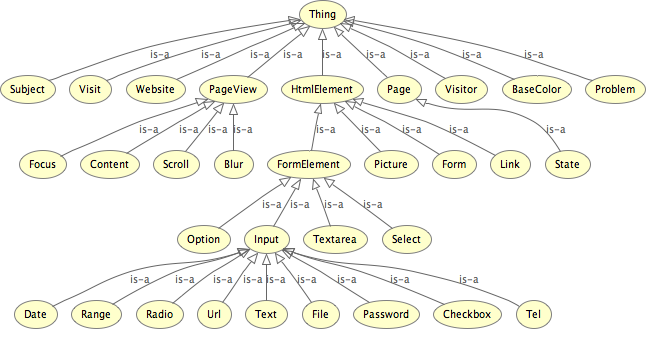
\includegraphics[width=0.7\textwidth]{figures/tbox}
\label{fig:onto}
\end{figure}

Außerdem wurde der Graph um die Konzepte der Besucherdaten erweitert.
Der vorherige Converte war wenig modular und umfasste ca. 2000 Zeilen in nur 4 Dateien.
Die Konfiguration war im Code eingebettet, sodass der Code insgesamt nciht sehr gut wartbar ist.
Die Neuimplementierung sieht einen wesentlichen modulareren Aufbau vor, sodass Anpassungen in der Vorverarbeitung effizient einsetzbar ist.
Sie berücksichtigt außerdem die Transformation der Daten in die korrekten Datentypen (Integer, Decimal, Boolean, ...).
Das Grundvokabular ist komplett separat entwickelt und wird in die Konvertierung miteinbezogen.
Dadurch ist der Zugriff vereinfacht und mittels eigener Entwicklungstools die Ontologie als Graph darstellbar.
Trotz der vielen Anpassungen und Erweiterungen umfasst der Quellcode nun gerade mal ca. 900 Zeilen und 15 Klassen inkl. rudimentären Testcode.
Man kann das Tool mittels Kommandozeiletool (\ref{listing:cli}) ausführen oder in ein Ruby-Projekt als Bibliothek einbinden.

\lstinputlisting[breaklines=true,language=Bash, caption=Beispielnutzung des Kommandozeilentools,label=listing:cli]{listings/abrupt_usage.sh}

Die Implementierung durch einen Regelsatz ist eine anschauliche Vorgehensweise für das Auffinden von Problemen. 
Ohne die Vorverarbeitung des Converters sind der Arbeit allerdings aufgrund der Open World Assumption Grenzen gesetzt.
Für das Überwinden der Grenzen, die in einer offenen Weltannahme entstehen, müssen die Eingabedaten vor der Konvertierung als geschlossen angenommen werden um vernünftiges Hilfswissen zu generieren.
Nur so ist man mit OWL 2 RL in der Lage mit einem Regelsatz auf Probleme zu schließen.
Die Generierung von Regeln ist nicht immer ganz einfach, da mit der Beschreibungslogik eine abgespeckte Mächtigkeit zur Verfügung steht. 
Diese zwingen den Entwickler oft zu einer bestimmte Vorgehensweise.
Anders als in konventionellen Programmierparadigmen gibt es nur wenige Lösungswege.
Dafür ist das Regelwerk Bestandteil des OWL-Dokuments und ist als solches für Mensch und Maschine lesbar und einfach austauschbar.
Man spart und verteilt Rechenzeit, da das Schlussfolgern, die eigentliche Programmausführung, auf dem jeweiligen Rechner stattfinden kann.
Theortisch ist es sogar eine Parallelisierung möglich.
Der Converter muss in der Regel mit großen Dateien umgehen können.
In der Entwicklung wurden Webseitendaten mit über 300 KB und Besucherdaten aus mit über 2 MB verwendet.
Durch das Umwandeln und Ergänzen der Daten in das OWL-Dokument entsteht darus eine turtle-Datei mit über 30 MB.
Dies entspricht einer Vergrößerung der Daten um den Faktor 15.
Dementsprechend ist die momentane Verarbeitungszeit auch sehr lange.
Der Flaschenhals liegt bei der Serialisierung des RDF-Grpahen durch die Ruby-Bibliothek {}"rdf-raptor{}" \cite{rdf-raptor}.
Das Regelwerk ist noch relativ bescheiden und ausbaufähig.
Für die Datentyp-Regeln fehlen noch Schwellwerte.
Diese zu definieren ist nicht trivial, da Texte kontextbezogen unterschiedliche Ansprüche hervorbringen.
Die Inkonsitenz-Regeln dagegen bieten bereits eine weitgehend Abdeckung. 
In \cite{Brieger} wurde bereits eine Web-Benutzeroberfläche (GUI) gestaltet, die den (alten) Converter anwendet.
Für die neuen Erweiterungen, insbesondere der Einfluss der Besucherdaten ist diese GUI noch nicht vorbereitet.
Eine Konfigurationsmaske für die kontextbezogenen Schwellwerte wäre denkbar.
Das Reasoning über das Dokument ist im Projekt nicht berücksichtigt und wird derzeit über properitäre Software vollzogen.
Eine Hybrid-Lösung könnte eine geeignete Wahl sein um die jeweiligen Vorteile der Klassifizierungs-Strategien zu nutzen.
Um die Software zu einem Gesamtprodukt zu komplettieren, besteht die Herausforderung der Vereinigung von Crawler, Converter, Reasoner und einer Eingabe- und Ausgabemaske.

\nocite{url_dl_primer}

\bibliography{literature}
\bibliographystyle{alpha}

\end{document}
